% Options for packages loaded elsewhere
\PassOptionsToPackage{unicode}{hyperref}
\PassOptionsToPackage{hyphens}{url}
\PassOptionsToPackage{dvipsnames,svgnames,x11names}{xcolor}
%
\documentclass[
  11pt,
]{article}
\title{Introduction to Meta-Analysis with R}
\usepackage{etoolbox}
\makeatletter
\providecommand{\subtitle}[1]{% add subtitle to \maketitle
  \apptocmd{\@title}{\par {\large #1 \par}}{}{}
}
\makeatother
\subtitle{KITE-Trainees Workshop Series}
\author{Mohammadreza Amiri, PhD MSc BA}
\date{2021-10-26}

\usepackage{amsmath,amssymb}
\usepackage{lmodern}
\usepackage{iftex}
\ifPDFTeX
  \usepackage[T1]{fontenc}
  \usepackage[utf8]{inputenc}
  \usepackage{textcomp} % provide euro and other symbols
\else % if luatex or xetex
  \usepackage{unicode-math}
  \defaultfontfeatures{Scale=MatchLowercase}
  \defaultfontfeatures[\rmfamily]{Ligatures=TeX,Scale=1}
\fi
% Use upquote if available, for straight quotes in verbatim environments
\IfFileExists{upquote.sty}{\usepackage{upquote}}{}
\IfFileExists{microtype.sty}{% use microtype if available
  \usepackage[]{microtype}
  \UseMicrotypeSet[protrusion]{basicmath} % disable protrusion for tt fonts
}{}
\makeatletter
\@ifundefined{KOMAClassName}{% if non-KOMA class
  \IfFileExists{parskip.sty}{%
    \usepackage{parskip}
  }{% else
    \setlength{\parindent}{0pt}
    \setlength{\parskip}{6pt plus 2pt minus 1pt}}
}{% if KOMA class
  \KOMAoptions{parskip=half}}
\makeatother
\usepackage{xcolor}
\IfFileExists{xurl.sty}{\usepackage{xurl}}{} % add URL line breaks if available
\IfFileExists{bookmark.sty}{\usepackage{bookmark}}{\usepackage{hyperref}}
\hypersetup{
  pdftitle={Introduction to Meta-Analysis with R},
  pdfauthor={Mohammadreza Amiri, PhD MSc BA},
  colorlinks=true,
  linkcolor={blue},
  filecolor={Maroon},
  citecolor={blue},
  urlcolor={blue},
  pdfcreator={LaTeX via pandoc}}
\urlstyle{same} % disable monospaced font for URLs
\usepackage[margin=1in]{geometry}
\usepackage{color}
\usepackage{fancyvrb}
\newcommand{\VerbBar}{|}
\newcommand{\VERB}{\Verb[commandchars=\\\{\}]}
\DefineVerbatimEnvironment{Highlighting}{Verbatim}{commandchars=\\\{\}}
% Add ',fontsize=\small' for more characters per line
\usepackage{framed}
\definecolor{shadecolor}{RGB}{248,248,248}
\newenvironment{Shaded}{\begin{snugshade}}{\end{snugshade}}
\newcommand{\AlertTok}[1]{\textcolor[rgb]{0.94,0.16,0.16}{#1}}
\newcommand{\AnnotationTok}[1]{\textcolor[rgb]{0.56,0.35,0.01}{\textbf{\textit{#1}}}}
\newcommand{\AttributeTok}[1]{\textcolor[rgb]{0.77,0.63,0.00}{#1}}
\newcommand{\BaseNTok}[1]{\textcolor[rgb]{0.00,0.00,0.81}{#1}}
\newcommand{\BuiltInTok}[1]{#1}
\newcommand{\CharTok}[1]{\textcolor[rgb]{0.31,0.60,0.02}{#1}}
\newcommand{\CommentTok}[1]{\textcolor[rgb]{0.56,0.35,0.01}{\textit{#1}}}
\newcommand{\CommentVarTok}[1]{\textcolor[rgb]{0.56,0.35,0.01}{\textbf{\textit{#1}}}}
\newcommand{\ConstantTok}[1]{\textcolor[rgb]{0.00,0.00,0.00}{#1}}
\newcommand{\ControlFlowTok}[1]{\textcolor[rgb]{0.13,0.29,0.53}{\textbf{#1}}}
\newcommand{\DataTypeTok}[1]{\textcolor[rgb]{0.13,0.29,0.53}{#1}}
\newcommand{\DecValTok}[1]{\textcolor[rgb]{0.00,0.00,0.81}{#1}}
\newcommand{\DocumentationTok}[1]{\textcolor[rgb]{0.56,0.35,0.01}{\textbf{\textit{#1}}}}
\newcommand{\ErrorTok}[1]{\textcolor[rgb]{0.64,0.00,0.00}{\textbf{#1}}}
\newcommand{\ExtensionTok}[1]{#1}
\newcommand{\FloatTok}[1]{\textcolor[rgb]{0.00,0.00,0.81}{#1}}
\newcommand{\FunctionTok}[1]{\textcolor[rgb]{0.00,0.00,0.00}{#1}}
\newcommand{\ImportTok}[1]{#1}
\newcommand{\InformationTok}[1]{\textcolor[rgb]{0.56,0.35,0.01}{\textbf{\textit{#1}}}}
\newcommand{\KeywordTok}[1]{\textcolor[rgb]{0.13,0.29,0.53}{\textbf{#1}}}
\newcommand{\NormalTok}[1]{#1}
\newcommand{\OperatorTok}[1]{\textcolor[rgb]{0.81,0.36,0.00}{\textbf{#1}}}
\newcommand{\OtherTok}[1]{\textcolor[rgb]{0.56,0.35,0.01}{#1}}
\newcommand{\PreprocessorTok}[1]{\textcolor[rgb]{0.56,0.35,0.01}{\textit{#1}}}
\newcommand{\RegionMarkerTok}[1]{#1}
\newcommand{\SpecialCharTok}[1]{\textcolor[rgb]{0.00,0.00,0.00}{#1}}
\newcommand{\SpecialStringTok}[1]{\textcolor[rgb]{0.31,0.60,0.02}{#1}}
\newcommand{\StringTok}[1]{\textcolor[rgb]{0.31,0.60,0.02}{#1}}
\newcommand{\VariableTok}[1]{\textcolor[rgb]{0.00,0.00,0.00}{#1}}
\newcommand{\VerbatimStringTok}[1]{\textcolor[rgb]{0.31,0.60,0.02}{#1}}
\newcommand{\WarningTok}[1]{\textcolor[rgb]{0.56,0.35,0.01}{\textbf{\textit{#1}}}}
\usepackage{longtable,booktabs,array}
\usepackage{calc} % for calculating minipage widths
% Correct order of tables after \paragraph or \subparagraph
\usepackage{etoolbox}
\makeatletter
\patchcmd\longtable{\par}{\if@noskipsec\mbox{}\fi\par}{}{}
\makeatother
% Allow footnotes in longtable head/foot
\IfFileExists{footnotehyper.sty}{\usepackage{footnotehyper}}{\usepackage{footnote}}
\makesavenoteenv{longtable}
\usepackage{graphicx}
\makeatletter
\def\maxwidth{\ifdim\Gin@nat@width>\linewidth\linewidth\else\Gin@nat@width\fi}
\def\maxheight{\ifdim\Gin@nat@height>\textheight\textheight\else\Gin@nat@height\fi}
\makeatother
% Scale images if necessary, so that they will not overflow the page
% margins by default, and it is still possible to overwrite the defaults
% using explicit options in \includegraphics[width, height, ...]{}
\setkeys{Gin}{width=\maxwidth,height=\maxheight,keepaspectratio}
% Set default figure placement to htbp
\makeatletter
\def\fps@figure{htbp}
\makeatother
\setlength{\emergencystretch}{3em} % prevent overfull lines
\providecommand{\tightlist}{%
  \setlength{\itemsep}{0pt}\setlength{\parskip}{0pt}}
\setcounter{secnumdepth}{5}
\newlength{\cslhangindent}
\setlength{\cslhangindent}{1.5em}
\newlength{\csllabelwidth}
\setlength{\csllabelwidth}{3em}
\newlength{\cslentryspacingunit} % times entry-spacing
\setlength{\cslentryspacingunit}{\parskip}
\newenvironment{CSLReferences}[2] % #1 hanging-ident, #2 entry spacing
 {% don't indent paragraphs
  \setlength{\parindent}{0pt}
  % turn on hanging indent if param 1 is 1
  \ifodd #1
  \let\oldpar\par
  \def\par{\hangindent=\cslhangindent\oldpar}
  \fi
  % set entry spacing
  \setlength{\parskip}{#2\cslentryspacingunit}
 }%
 {}
\usepackage{calc}
\newcommand{\CSLBlock}[1]{#1\hfill\break}
\newcommand{\CSLLeftMargin}[1]{\parbox[t]{\csllabelwidth}{#1}}
\newcommand{\CSLRightInline}[1]{\parbox[t]{\linewidth - \csllabelwidth}{#1}\break}
\newcommand{\CSLIndent}[1]{\hspace{\cslhangindent}#1}
\ifLuaTeX
  \usepackage{selnolig}  % disable illegal ligatures
\fi

\begin{document}
\maketitle

{
\hypersetup{linkcolor=}
\setcounter{tocdepth}{2}
\tableofcontents
}
\hypertarget{making-everything-ready}{%
\section{Making Everything Ready}\label{making-everything-ready}}

Visit this \href{https://learnr-examples.shinyapps.io/ex-setup-r/}{link} to find out how to install R, RStudio IDE, and install R packages.

\hypertarget{r}{%
\subsection{R}\label{r}}

R is a free software environment for statistical computing and graphics. R software can be downloaded \href{https://www.r-project.org/}{here}. The most recent version of R is 4.1.1 (Kick Things) and has been released on 2021-08-10. However, some packages that I frequently use do not support the newest version of R. Facilitating this issue, I use version 3.6.3 on my system. Nonetheless, you are able to install and use multiple version of R on your system and using RStudio you can switch back and forth to any version of R based on your needs. To get help using R access their webpage \href{https://www.r-project.org/help.html}{here}.

\hypertarget{rstudio}{%
\subsection{RStudio}\label{rstudio}}

RStudio's mission is to create free and open-source software for data science, scientific research, and technical communication. Inspired by innovators in science, education, government, and industry, RStudio develops free and open tools for R, and enterprise-ready professional products for teams who use both R and Python, to scale and share their work. RStudio Integrated development environment (IDE) can be downloaded \href{https://www.rstudio.com/products/rstudio/download/}{here}. We are using RStudio for this workshop.

\hypertarget{what-is-a-meta-analysis-ma}{%
\section{What is a meta-analysis (MA)?}\label{what-is-a-meta-analysis-ma}}

\hypertarget{definition}{%
\subsection{Definition}\label{definition}}

The following definitions summarize the MA statistical technique:

\begin{quote}
``Analysis of analyses'' (\protect\hyperlink{ref-glass1976}{Glass, 1976})
\end{quote}

\begin{quote}
``Meta-analysis can be understood as a form of survey research in which research reports, rather than people, are surveyed.'' (\protect\hyperlink{ref-lipsey2001}{Lipsey \& Wilson, 2001})
\end{quote}

\hypertarget{the-best-packages-to-conduct-a-ma}{%
\section{The Best packages to Conduct a MA}\label{the-best-packages-to-conduct-a-ma}}

In my opinion, the best packages are \href{https://github.com/guido-s/meta/}{meta} (for ease of use and has a \href{https://www.springer.com/gp/book/9783319214153}{book}) and \href{https://www.metafor-project.org/doku.php}{metafor} for best documentation (after installation type \texttt{vignette("metafor")}).

\hypertarget{data-preparation}{%
\section{Data Preparation}\label{data-preparation}}

Loading required packages (don't forget to install the packages first if you have not done so):

Let's view the data for this session:

\begin{Shaded}
\begin{Highlighting}[]
\NormalTok{dat }\OtherTok{\textless{}{-}}\NormalTok{ dat.bcg}

\NormalTok{knitr}\SpecialCharTok{::}\FunctionTok{kable}\NormalTok{(dat)}
\end{Highlighting}
\end{Shaded}

\begin{tabular}{r|l|r|r|r|r|r|r|l}
\hline
trial & author & year & tpos & tneg & cpos & cneg & ablat & alloc\\
\hline
1 & Aronson & 1948 & 4 & 119 & 11 & 128 & 44 & random\\
\hline
2 & Ferguson \& Simes & 1949 & 6 & 300 & 29 & 274 & 55 & random\\
\hline
3 & Rosenthal et al & 1960 & 3 & 228 & 11 & 209 & 42 & random\\
\hline
4 & Hart \& Sutherland & 1977 & 62 & 13536 & 248 & 12619 & 52 & random\\
\hline
5 & Frimodt-Moller et al & 1973 & 33 & 5036 & 47 & 5761 & 13 & alternate\\
\hline
6 & Stein \& Aronson & 1953 & 180 & 1361 & 372 & 1079 & 44 & alternate\\
\hline
7 & Vandiviere et al & 1973 & 8 & 2537 & 10 & 619 & 19 & random\\
\hline
8 & TPT Madras & 1980 & 505 & 87886 & 499 & 87892 & 13 & random\\
\hline
9 & Coetzee \& Berjak & 1968 & 29 & 7470 & 45 & 7232 & 27 & random\\
\hline
10 & Rosenthal et al & 1961 & 17 & 1699 & 65 & 1600 & 42 & systematic\\
\hline
11 & Comstock et al & 1974 & 186 & 50448 & 141 & 27197 & 18 & systematic\\
\hline
12 & Comstock \& Webster & 1969 & 5 & 2493 & 3 & 2338 & 33 & systematic\\
\hline
13 & Comstock et al & 1976 & 27 & 16886 & 29 & 17825 & 33 & systematic\\
\hline
\end{tabular}

Now we need to calculate the log risk ratios and corresponding sampling variances (and use the `slab' argument to store study labels as part of the data frame):

\begin{Shaded}
\begin{Highlighting}[]
\NormalTok{ex1data }\OtherTok{\textless{}{-}} \FunctionTok{escalc}\NormalTok{(}\AttributeTok{measure =} \StringTok{"RR"}\NormalTok{, }\AttributeTok{ai =}\NormalTok{ tpos, }\AttributeTok{bi =}\NormalTok{ tneg, }\AttributeTok{ci =}\NormalTok{ cpos,}
    \AttributeTok{di =}\NormalTok{ cneg, }\AttributeTok{data =}\NormalTok{ dat, }\AttributeTok{slab =} \FunctionTok{paste}\NormalTok{(author, year, }\AttributeTok{sep =} \StringTok{", "}\NormalTok{))}

\CommentTok{\# set\_flextable\_defaults( font.family = \textquotesingle{}Arial\textquotesingle{}, font.size}
\CommentTok{\# = 10, font.color = \textquotesingle{}black\textquotesingle{}, table.layout = \textquotesingle{}autofit\textquotesingle{},}
\CommentTok{\# digits = 3, theme\_fun = \textquotesingle{}\textquotesingle{} )}

\NormalTok{ex1data }\SpecialCharTok{\%\textgreater{}\%}
    \FunctionTok{select}\NormalTok{(trial, author, year, yi, vi) }\SpecialCharTok{\%\textgreater{}\%}
    \FunctionTok{head}\NormalTok{(}\DecValTok{5}\NormalTok{) }\SpecialCharTok{\%\textgreater{}\%}
    \FunctionTok{flextable}\NormalTok{() }\SpecialCharTok{\%\textgreater{}\%}
    \FunctionTok{set\_caption}\NormalTok{(}\StringTok{"Effect size and variance"}\NormalTok{) }\SpecialCharTok{\%\textgreater{}\%}
    \FunctionTok{set\_table\_properties}\NormalTok{(}\AttributeTok{layout =} \StringTok{"autofit"}\NormalTok{) }\SpecialCharTok{\%\textgreater{}\%}
    \FunctionTok{colformat\_double}\NormalTok{(}\AttributeTok{digits =} \DecValTok{3}\NormalTok{) }\SpecialCharTok{\%\textgreater{}\%}
    \FunctionTok{theme\_booktabs}\NormalTok{()}
\end{Highlighting}
\end{Shaded}

\providecommand{\docline}[3]{\noalign{\global\setlength{\arrayrulewidth}{#1}}\arrayrulecolor[HTML]{#2}\cline{#3}}

\setlength{\tabcolsep}{2pt}

\renewcommand*{\arraystretch}{1.5}

\begin{longtable}[c]{ccccc}

\caption{Effect size and variance
}\label{tab:data-preparation}\\

\hhline{>{\arrayrulecolor[HTML]{666666}\global\arrayrulewidth=2pt}->{\arrayrulecolor[HTML]{666666}\global\arrayrulewidth=2pt}->{\arrayrulecolor[HTML]{666666}\global\arrayrulewidth=2pt}->{\arrayrulecolor[HTML]{666666}\global\arrayrulewidth=2pt}->{\arrayrulecolor[HTML]{666666}\global\arrayrulewidth=2pt}-}

\multicolumn{1}{!{\color[HTML]{000000}\vrule width 0pt}>{}r}{\fontsize{11}{11}\selectfont{\textcolor[HTML]{000000}{trial}}} & \multicolumn{1}{!{\color[HTML]{000000}\vrule width 0pt}>{}l}{\fontsize{11}{11}\selectfont{\textcolor[HTML]{000000}{author}}} & \multicolumn{1}{!{\color[HTML]{000000}\vrule width 0pt}>{}r}{\fontsize{11}{11}\selectfont{\textcolor[HTML]{000000}{year}}} & \multicolumn{1}{!{\color[HTML]{000000}\vrule width 0pt}>{}r}{\fontsize{11}{11}\selectfont{\textcolor[HTML]{000000}{yi}}} & \multicolumn{1}{!{\color[HTML]{000000}\vrule width 0pt}>{}r!{\color[HTML]{000000}\vrule width 0pt}}{\fontsize{11}{11}\selectfont{\textcolor[HTML]{000000}{vi}}} \\

\hhline{>{\arrayrulecolor[HTML]{666666}\global\arrayrulewidth=2pt}->{\arrayrulecolor[HTML]{666666}\global\arrayrulewidth=2pt}->{\arrayrulecolor[HTML]{666666}\global\arrayrulewidth=2pt}->{\arrayrulecolor[HTML]{666666}\global\arrayrulewidth=2pt}->{\arrayrulecolor[HTML]{666666}\global\arrayrulewidth=2pt}-}

\endfirsthead

\hhline{>{\arrayrulecolor[HTML]{666666}\global\arrayrulewidth=2pt}->{\arrayrulecolor[HTML]{666666}\global\arrayrulewidth=2pt}->{\arrayrulecolor[HTML]{666666}\global\arrayrulewidth=2pt}->{\arrayrulecolor[HTML]{666666}\global\arrayrulewidth=2pt}->{\arrayrulecolor[HTML]{666666}\global\arrayrulewidth=2pt}-}

\multicolumn{1}{!{\color[HTML]{000000}\vrule width 0pt}>{}r}{\fontsize{11}{11}\selectfont{\textcolor[HTML]{000000}{trial}}} & \multicolumn{1}{!{\color[HTML]{000000}\vrule width 0pt}>{}l}{\fontsize{11}{11}\selectfont{\textcolor[HTML]{000000}{author}}} & \multicolumn{1}{!{\color[HTML]{000000}\vrule width 0pt}>{}r}{\fontsize{11}{11}\selectfont{\textcolor[HTML]{000000}{year}}} & \multicolumn{1}{!{\color[HTML]{000000}\vrule width 0pt}>{}r}{\fontsize{11}{11}\selectfont{\textcolor[HTML]{000000}{yi}}} & \multicolumn{1}{!{\color[HTML]{000000}\vrule width 0pt}>{}r!{\color[HTML]{000000}\vrule width 0pt}}{\fontsize{11}{11}\selectfont{\textcolor[HTML]{000000}{vi}}} \\

\hhline{>{\arrayrulecolor[HTML]{666666}\global\arrayrulewidth=2pt}->{\arrayrulecolor[HTML]{666666}\global\arrayrulewidth=2pt}->{\arrayrulecolor[HTML]{666666}\global\arrayrulewidth=2pt}->{\arrayrulecolor[HTML]{666666}\global\arrayrulewidth=2pt}->{\arrayrulecolor[HTML]{666666}\global\arrayrulewidth=2pt}-}\endhead



\multicolumn{1}{!{\color[HTML]{000000}\vrule width 0pt}>{}r}{\fontsize{11}{11}\selectfont{\textcolor[HTML]{000000}{1}}} & \multicolumn{1}{!{\color[HTML]{000000}\vrule width 0pt}>{}l}{\fontsize{11}{11}\selectfont{\textcolor[HTML]{000000}{Aronson}}} & \multicolumn{1}{!{\color[HTML]{000000}\vrule width 0pt}>{}r}{\fontsize{11}{11}\selectfont{\textcolor[HTML]{000000}{1,948}}} & \multicolumn{1}{!{\color[HTML]{000000}\vrule width 0pt}>{}r}{\fontsize{11}{11}\selectfont{\textcolor[HTML]{000000}{-0.889}}} & \multicolumn{1}{!{\color[HTML]{000000}\vrule width 0pt}>{}r!{\color[HTML]{000000}\vrule width 0pt}}{\fontsize{11}{11}\selectfont{\textcolor[HTML]{000000}{0.326}}} \\





\multicolumn{1}{!{\color[HTML]{000000}\vrule width 0pt}>{}r}{\fontsize{11}{11}\selectfont{\textcolor[HTML]{000000}{2}}} & \multicolumn{1}{!{\color[HTML]{000000}\vrule width 0pt}>{}l}{\fontsize{11}{11}\selectfont{\textcolor[HTML]{000000}{Ferguson\ \&\ Simes}}} & \multicolumn{1}{!{\color[HTML]{000000}\vrule width 0pt}>{}r}{\fontsize{11}{11}\selectfont{\textcolor[HTML]{000000}{1,949}}} & \multicolumn{1}{!{\color[HTML]{000000}\vrule width 0pt}>{}r}{\fontsize{11}{11}\selectfont{\textcolor[HTML]{000000}{-1.585}}} & \multicolumn{1}{!{\color[HTML]{000000}\vrule width 0pt}>{}r!{\color[HTML]{000000}\vrule width 0pt}}{\fontsize{11}{11}\selectfont{\textcolor[HTML]{000000}{0.195}}} \\





\multicolumn{1}{!{\color[HTML]{000000}\vrule width 0pt}>{}r}{\fontsize{11}{11}\selectfont{\textcolor[HTML]{000000}{3}}} & \multicolumn{1}{!{\color[HTML]{000000}\vrule width 0pt}>{}l}{\fontsize{11}{11}\selectfont{\textcolor[HTML]{000000}{Rosenthal\ et\ al}}} & \multicolumn{1}{!{\color[HTML]{000000}\vrule width 0pt}>{}r}{\fontsize{11}{11}\selectfont{\textcolor[HTML]{000000}{1,960}}} & \multicolumn{1}{!{\color[HTML]{000000}\vrule width 0pt}>{}r}{\fontsize{11}{11}\selectfont{\textcolor[HTML]{000000}{-1.348}}} & \multicolumn{1}{!{\color[HTML]{000000}\vrule width 0pt}>{}r!{\color[HTML]{000000}\vrule width 0pt}}{\fontsize{11}{11}\selectfont{\textcolor[HTML]{000000}{0.415}}} \\





\multicolumn{1}{!{\color[HTML]{000000}\vrule width 0pt}>{}r}{\fontsize{11}{11}\selectfont{\textcolor[HTML]{000000}{4}}} & \multicolumn{1}{!{\color[HTML]{000000}\vrule width 0pt}>{}l}{\fontsize{11}{11}\selectfont{\textcolor[HTML]{000000}{Hart\ \&\ Sutherland}}} & \multicolumn{1}{!{\color[HTML]{000000}\vrule width 0pt}>{}r}{\fontsize{11}{11}\selectfont{\textcolor[HTML]{000000}{1,977}}} & \multicolumn{1}{!{\color[HTML]{000000}\vrule width 0pt}>{}r}{\fontsize{11}{11}\selectfont{\textcolor[HTML]{000000}{-1.442}}} & \multicolumn{1}{!{\color[HTML]{000000}\vrule width 0pt}>{}r!{\color[HTML]{000000}\vrule width 0pt}}{\fontsize{11}{11}\selectfont{\textcolor[HTML]{000000}{0.020}}} \\





\multicolumn{1}{!{\color[HTML]{000000}\vrule width 0pt}>{}r}{\fontsize{11}{11}\selectfont{\textcolor[HTML]{000000}{5}}} & \multicolumn{1}{!{\color[HTML]{000000}\vrule width 0pt}>{}l}{\fontsize{11}{11}\selectfont{\textcolor[HTML]{000000}{Frimodt-Moller\ et\ al}}} & \multicolumn{1}{!{\color[HTML]{000000}\vrule width 0pt}>{}r}{\fontsize{11}{11}\selectfont{\textcolor[HTML]{000000}{1,973}}} & \multicolumn{1}{!{\color[HTML]{000000}\vrule width 0pt}>{}r}{\fontsize{11}{11}\selectfont{\textcolor[HTML]{000000}{-0.218}}} & \multicolumn{1}{!{\color[HTML]{000000}\vrule width 0pt}>{}r!{\color[HTML]{000000}\vrule width 0pt}}{\fontsize{11}{11}\selectfont{\textcolor[HTML]{000000}{0.051}}} \\

\hhline{>{\arrayrulecolor[HTML]{666666}\global\arrayrulewidth=2pt}->{\arrayrulecolor[HTML]{666666}\global\arrayrulewidth=2pt}->{\arrayrulecolor[HTML]{666666}\global\arrayrulewidth=2pt}->{\arrayrulecolor[HTML]{666666}\global\arrayrulewidth=2pt}->{\arrayrulecolor[HTML]{666666}\global\arrayrulewidth=2pt}-}



\end{longtable}

Effect size (\emph{yi}): Log(RR)

Variance of effect size (\emph{vi}): Variance Log(RR)

Note (\protect\hyperlink{ref-metafor}{Viechtbauer, 2010}):

In various fields (such as the health and medical sciences), the response variable measured is often dichotomous (binary), so that the data from a study comparing two different groups can be expressed in terms of a table, such as:

\begin{longtable}[]{@{}llll@{}}
\caption{Example of dichotomous outcomes}\tabularnewline
\toprule
& Outcome 1 & Outcome 2 & Total \\
\midrule
\endfirsthead
\toprule
& Outcome 1 & Outcome 2 & Total \\
\midrule
\endhead
Group 1 & ai & bi & n1i \\
Group 2 & ci & di & n2i \\
\bottomrule
\end{longtable}

where ai, bi, ci, and di denote the cell frequencies (i.e., the number of people falling into a particular category) and n1i and n2i are the row totals (i.e., the group sizes).

For example, in a set of randomized clinical trials, group 1 and group 2 may refer to the treatment and placebo/control group, respectively, with outcome 1 denoting some event of interest (e.g., death, complications, failure to improve under the treatment) and outcome 2 its complement. Similarly, in a set of cohort studies, group 1 and group 2 may denote those who engage in and those who do not engage in a potentially harmful behavior (e.g., smoking), with outcome 1 denoting the development of a particular disease (e.g., lung cancer) during the follow-up period. Finally, in a set of case-control studies, group 1 and group 2 may refer to those with the disease (i.e., cases) and those free of the disease (i.e., controls), with outcome 1 denoting, for example, exposure to some environmental risk factor in the past and outcome 2 non-exposure. Note that in all of these examples, the stratified sampling scheme fixes the row totals (i.e., the group sizes) by design.

A meta-analysis of studies reporting results in terms of tables can be based on one of several different outcome measures, including the risk ratio (also called the relative risk), the odds ratio, the risk difference, and the arcsine square root transformed risk difference (\protect\hyperlink{ref-Ruxfccker2009}{Rücker et al., 2009}). For any of these outcome measures, one needs to specify the cell frequencies via the ai, bi, ci, and di arguments (or alternatively, one can use the ai, ci, n1i, and n2i arguments).

The options for the measure argument are then:

``RR'' for the log risk ratio,

``OR'' for the log odds ratio,

``RD'' for the risk difference,

``AS'' for the arcsine square root transformed risk difference (\protect\hyperlink{ref-Ruxfccker2009}{Rücker et al., 2009}),

``PETO'' for the log odds ratio estimated with Peto's method (\protect\hyperlink{ref-Yusuf1985}{Yusuf et al., 1985}).

Note that the log is taken of the risk ratio and the odds ratio, which makes these outcome measures symmetric around 0 and yields corresponding sampling distributions that are closer to normality. Also, when multiplied by 2, the arcsine square root transformed risk difference is actually identical to Cohen's h (\protect\hyperlink{ref-cohen1977}{Cohen, 1977}).

\hypertarget{hands-on-practice}{%
\section{Hands-on practice}\label{hands-on-practice}}

\hypertarget{forest-plot-using-metafor-package}{%
\subsection{Forest Plot Using metafor Package}\label{forest-plot-using-metafor-package}}

\hypertarget{unordered-forest-plot}{%
\subsubsection{Unordered Forest Plot}\label{unordered-forest-plot}}

\begin{Shaded}
\begin{Highlighting}[]
\CommentTok{\# Fitting a random{-}effects model}
\NormalTok{res }\OtherTok{\textless{}{-}} \FunctionTok{rma}\NormalTok{(yi, vi, }\AttributeTok{data =}\NormalTok{ ex1data)}


\CommentTok{\# Forest plot combined with (necessary) annotations}
\FunctionTok{forest}\NormalTok{(res, }\AttributeTok{atransf =}\NormalTok{ exp, }\AttributeTok{at =} \FunctionTok{log}\NormalTok{(}\FunctionTok{c}\NormalTok{(}\FloatTok{0.05}\NormalTok{, }\FloatTok{0.25}\NormalTok{, }\DecValTok{1}\NormalTok{, }\DecValTok{4}\NormalTok{)), }\AttributeTok{xlim =} \FunctionTok{c}\NormalTok{(}\SpecialCharTok{{-}}\DecValTok{16}\NormalTok{,}
    \DecValTok{6}\NormalTok{), }\AttributeTok{ilab =} \FunctionTok{cbind}\NormalTok{(dat.bcg}\SpecialCharTok{$}\NormalTok{tpos, dat.bcg}\SpecialCharTok{$}\NormalTok{tneg, dat.bcg}\SpecialCharTok{$}\NormalTok{cpos,}
\NormalTok{    dat.bcg}\SpecialCharTok{$}\NormalTok{cneg), }\AttributeTok{ilab.xpos =} \FunctionTok{c}\NormalTok{(}\SpecialCharTok{{-}}\FloatTok{9.5}\NormalTok{, }\SpecialCharTok{{-}}\DecValTok{8}\NormalTok{, }\SpecialCharTok{{-}}\DecValTok{6}\NormalTok{, }\SpecialCharTok{{-}}\FloatTok{4.5}\NormalTok{), }\AttributeTok{cex =} \FloatTok{0.75}\NormalTok{,}
    \AttributeTok{header =} \StringTok{"Author(s) and Year"}\NormalTok{, }\AttributeTok{mlab =} \StringTok{""}\NormalTok{)}

\NormalTok{op }\OtherTok{\textless{}{-}} \FunctionTok{par}\NormalTok{(}\AttributeTok{cex =} \FloatTok{0.75}\NormalTok{, }\AttributeTok{font =} \DecValTok{2}\NormalTok{)}

\FunctionTok{text}\NormalTok{(}\FunctionTok{c}\NormalTok{(}\SpecialCharTok{{-}}\FloatTok{9.5}\NormalTok{, }\SpecialCharTok{{-}}\DecValTok{8}\NormalTok{, }\SpecialCharTok{{-}}\DecValTok{6}\NormalTok{, }\SpecialCharTok{{-}}\FloatTok{4.5}\NormalTok{), }\DecValTok{15}\NormalTok{, }\FunctionTok{c}\NormalTok{(}\StringTok{"TB+"}\NormalTok{, }\StringTok{"TB{-}"}\NormalTok{, }\StringTok{"TB+"}\NormalTok{, }\StringTok{"TB{-}"}\NormalTok{))}

\FunctionTok{text}\NormalTok{(}\FunctionTok{c}\NormalTok{(}\SpecialCharTok{{-}}\FloatTok{8.75}\NormalTok{, }\SpecialCharTok{{-}}\FloatTok{5.25}\NormalTok{), }\DecValTok{16}\NormalTok{, }\FunctionTok{c}\NormalTok{(}\StringTok{"Vaccinated"}\NormalTok{, }\StringTok{"Control"}\NormalTok{))}

\FunctionTok{par}\NormalTok{(op)}


\CommentTok{\# add text with Q{-}value, dfs, p{-}value, and I\^{}2 statistic}
\FunctionTok{text}\NormalTok{(}\SpecialCharTok{{-}}\DecValTok{16}\NormalTok{, }\SpecialCharTok{{-}}\DecValTok{1}\NormalTok{, }\AttributeTok{pos =} \DecValTok{4}\NormalTok{, }\AttributeTok{cex =} \FloatTok{0.75}\NormalTok{, }\FunctionTok{bquote}\NormalTok{(}\FunctionTok{paste}\NormalTok{(}\StringTok{"RE Model (Q = "}\NormalTok{,}
\NormalTok{    .(}\FunctionTok{formatC}\NormalTok{(res}\SpecialCharTok{$}\NormalTok{QE, }\AttributeTok{digits =} \DecValTok{2}\NormalTok{, }\AttributeTok{format =} \StringTok{"f"}\NormalTok{)), }\StringTok{", df = "}\NormalTok{,}
\NormalTok{    .(res}\SpecialCharTok{$}\NormalTok{k }\SpecialCharTok{{-}}\NormalTok{ res}\SpecialCharTok{$}\NormalTok{p), }\StringTok{", p = "}\NormalTok{, .(}\FunctionTok{formatC}\NormalTok{(res}\SpecialCharTok{$}\NormalTok{QEp, }\AttributeTok{digits =} \DecValTok{2}\NormalTok{,}
        \AttributeTok{format =} \StringTok{"f"}\NormalTok{)), }\StringTok{"; "}\NormalTok{, I}\SpecialCharTok{\^{}}\DecValTok{2}\NormalTok{, }\StringTok{" = "}\NormalTok{, .(}\FunctionTok{formatC}\NormalTok{(res}\SpecialCharTok{$}\NormalTok{I2, }\AttributeTok{digits =} \DecValTok{1}\NormalTok{,}
        \AttributeTok{format =} \StringTok{"f"}\NormalTok{)), }\StringTok{"\%)"}\NormalTok{)))}
\end{Highlighting}
\end{Shaded}

\begin{figure}

{\centering 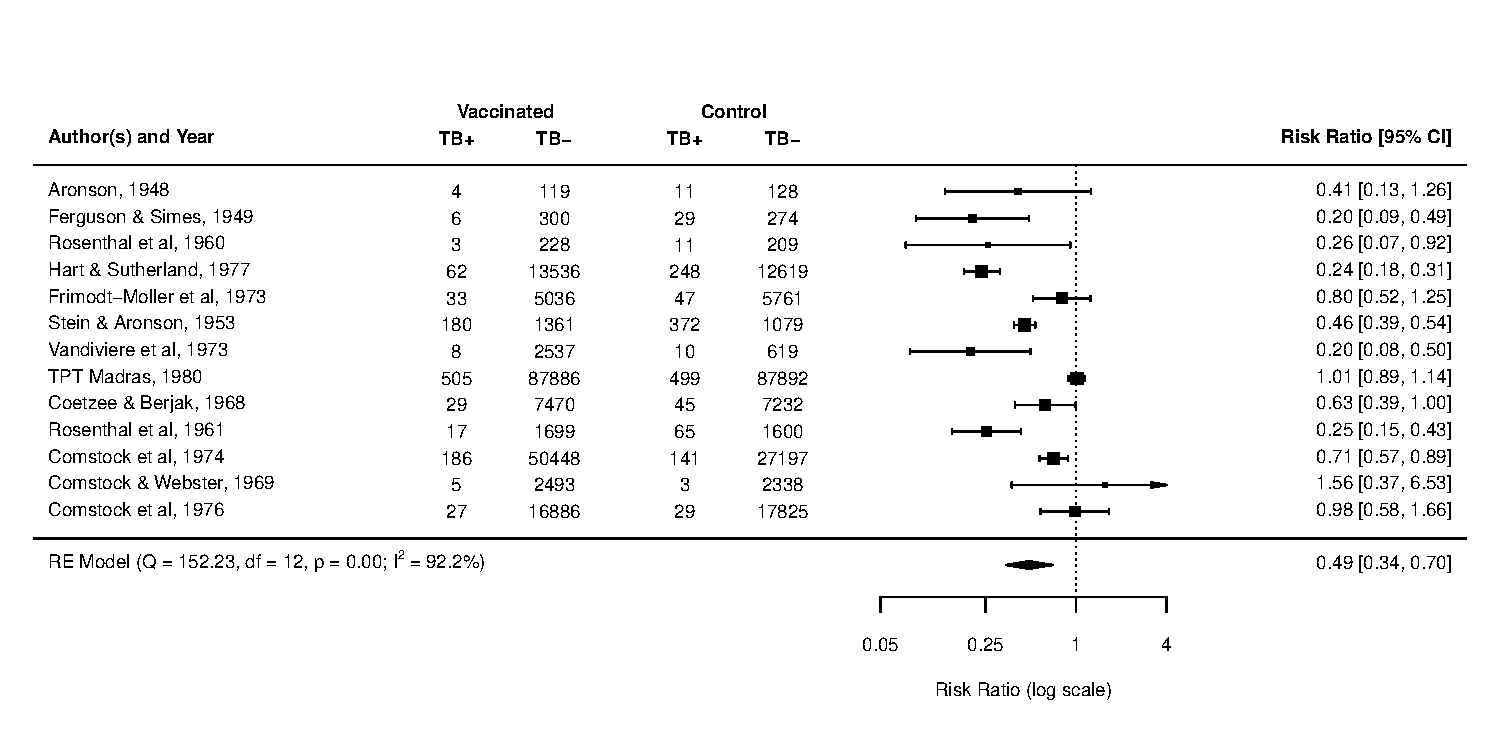
\includegraphics{IntroToMA_pdf_files/figure-latex/forest-plot-1} 

}

\caption{Unordered Forest Plot}\label{fig:forest-plot}
\end{figure}

\hypertarget{ordered-forest-plot}{%
\subsubsection{Ordered Forest Plot}\label{ordered-forest-plot}}

\begin{Shaded}
\begin{Highlighting}[]
\CommentTok{\# Fitting a random{-}effects model}
\NormalTok{res }\OtherTok{\textless{}{-}} \FunctionTok{rma}\NormalTok{(yi, vi, }\AttributeTok{data =}\NormalTok{ ex1data)}


\CommentTok{\# Forest plot combined with (necessary) annotations}
\FunctionTok{forest}\NormalTok{(res, }\AttributeTok{atransf =}\NormalTok{ exp, }\AttributeTok{at =} \FunctionTok{log}\NormalTok{(}\FunctionTok{c}\NormalTok{(}\FloatTok{0.05}\NormalTok{, }\FloatTok{0.25}\NormalTok{, }\DecValTok{1}\NormalTok{, }\DecValTok{4}\NormalTok{)), }\AttributeTok{xlim =} \FunctionTok{c}\NormalTok{(}\SpecialCharTok{{-}}\DecValTok{16}\NormalTok{,}
    \DecValTok{6}\NormalTok{), }\AttributeTok{ilab =} \FunctionTok{cbind}\NormalTok{(dat.bcg}\SpecialCharTok{$}\NormalTok{tpos, dat.bcg}\SpecialCharTok{$}\NormalTok{tneg, dat.bcg}\SpecialCharTok{$}\NormalTok{cpos,}
\NormalTok{    dat.bcg}\SpecialCharTok{$}\NormalTok{cneg), }\AttributeTok{ilab.xpos =} \FunctionTok{c}\NormalTok{(}\SpecialCharTok{{-}}\FloatTok{9.5}\NormalTok{, }\SpecialCharTok{{-}}\DecValTok{8}\NormalTok{, }\SpecialCharTok{{-}}\DecValTok{6}\NormalTok{, }\SpecialCharTok{{-}}\FloatTok{4.5}\NormalTok{), }\AttributeTok{cex =} \FloatTok{0.75}\NormalTok{,}
    \AttributeTok{header =} \StringTok{"Author(s) and Year"}\NormalTok{, }\AttributeTok{mlab =} \StringTok{""}\NormalTok{, }\AttributeTok{order =} \StringTok{"obs"}\NormalTok{)}

\NormalTok{op }\OtherTok{\textless{}{-}} \FunctionTok{par}\NormalTok{(}\AttributeTok{cex =} \FloatTok{0.75}\NormalTok{, }\AttributeTok{font =} \DecValTok{2}\NormalTok{)}

\FunctionTok{text}\NormalTok{(}\FunctionTok{c}\NormalTok{(}\SpecialCharTok{{-}}\FloatTok{9.5}\NormalTok{, }\SpecialCharTok{{-}}\DecValTok{8}\NormalTok{, }\SpecialCharTok{{-}}\DecValTok{6}\NormalTok{, }\SpecialCharTok{{-}}\FloatTok{4.5}\NormalTok{), }\DecValTok{15}\NormalTok{, }\FunctionTok{c}\NormalTok{(}\StringTok{"TB+"}\NormalTok{, }\StringTok{"TB{-}"}\NormalTok{, }\StringTok{"TB+"}\NormalTok{, }\StringTok{"TB{-}"}\NormalTok{))}

\FunctionTok{text}\NormalTok{(}\FunctionTok{c}\NormalTok{(}\SpecialCharTok{{-}}\FloatTok{8.75}\NormalTok{, }\SpecialCharTok{{-}}\FloatTok{5.25}\NormalTok{), }\DecValTok{16}\NormalTok{, }\FunctionTok{c}\NormalTok{(}\StringTok{"Vaccinated"}\NormalTok{, }\StringTok{"Control"}\NormalTok{))}

\FunctionTok{par}\NormalTok{(op)}


\CommentTok{\# add text with Q{-}value, dfs, p{-}value, and I\^{}2 statistic}
\FunctionTok{text}\NormalTok{(}\SpecialCharTok{{-}}\DecValTok{16}\NormalTok{, }\SpecialCharTok{{-}}\DecValTok{1}\NormalTok{, }\AttributeTok{pos =} \DecValTok{4}\NormalTok{, }\AttributeTok{cex =} \FloatTok{0.75}\NormalTok{, }\FunctionTok{bquote}\NormalTok{(}\FunctionTok{paste}\NormalTok{(}\StringTok{"RE Model (Q = "}\NormalTok{,}
\NormalTok{    .(}\FunctionTok{formatC}\NormalTok{(res}\SpecialCharTok{$}\NormalTok{QE, }\AttributeTok{digits =} \DecValTok{2}\NormalTok{, }\AttributeTok{format =} \StringTok{"f"}\NormalTok{)), }\StringTok{", df = "}\NormalTok{,}
\NormalTok{    .(res}\SpecialCharTok{$}\NormalTok{k }\SpecialCharTok{{-}}\NormalTok{ res}\SpecialCharTok{$}\NormalTok{p), }\StringTok{", p = "}\NormalTok{, .(}\FunctionTok{formatC}\NormalTok{(res}\SpecialCharTok{$}\NormalTok{QEp, }\AttributeTok{digits =} \DecValTok{2}\NormalTok{,}
        \AttributeTok{format =} \StringTok{"f"}\NormalTok{)), }\StringTok{"; "}\NormalTok{, I}\SpecialCharTok{\^{}}\DecValTok{2}\NormalTok{, }\StringTok{" = "}\NormalTok{, .(}\FunctionTok{formatC}\NormalTok{(res}\SpecialCharTok{$}\NormalTok{I2, }\AttributeTok{digits =} \DecValTok{1}\NormalTok{,}
        \AttributeTok{format =} \StringTok{"f"}\NormalTok{)), }\StringTok{"\%)"}\NormalTok{)))}
\end{Highlighting}
\end{Shaded}

\begin{figure}

{\centering 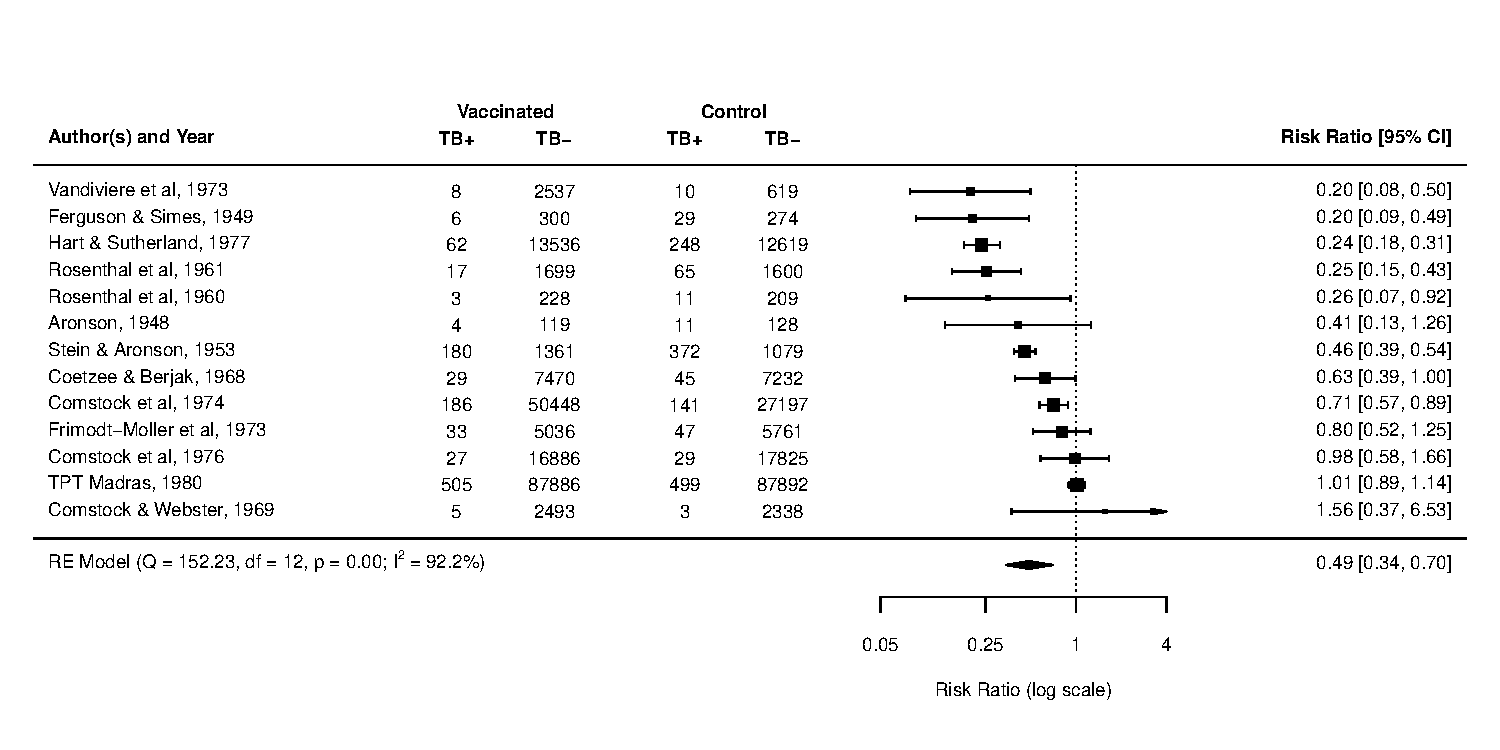
\includegraphics{IntroToMA_pdf_files/figure-latex/forest-plot-ordered-1} 

}

\caption{Ordered Forest Plot}\label{fig:forest-plot-ordered}
\end{figure}

\hypertarget{forest-plot-using-meta-package}{%
\subsection{Forest Plot Using meta Package}\label{forest-plot-using-meta-package}}

\begin{Shaded}
\begin{Highlighting}[]
\NormalTok{nfr }\OtherTok{\textless{}{-}} \FunctionTok{read.xlsx}\NormalTok{(}\AttributeTok{xlsxFile =} \StringTok{"NFR\_v\_Control\_final.xlsx"}\NormalTok{)}

\NormalTok{nfrModel }\OtherTok{\textless{}{-}} \FunctionTok{metacont}\NormalTok{(}\AttributeTok{data =}\NormalTok{ nfr, }\AttributeTok{n.e =}\NormalTok{ ss1, }\AttributeTok{mean.e =}\NormalTok{ m1, }\AttributeTok{sd.e =}\NormalTok{ sd1,}
    \AttributeTok{n.c =}\NormalTok{ ss2, }\AttributeTok{mean.c =}\NormalTok{ m2, }\AttributeTok{sd.c =}\NormalTok{ sd2, }\AttributeTok{studlab =}\NormalTok{ Study.Label,}
    \AttributeTok{sm =} \StringTok{"SMD"}\NormalTok{)}

\FunctionTok{forest}\NormalTok{(}\AttributeTok{x =}\NormalTok{ nfrModel, }\AttributeTok{comb.random =}\NormalTok{ F, }\AttributeTok{digits.mean =} \DecValTok{1}\NormalTok{, }\AttributeTok{digits.sd =} \DecValTok{1}\NormalTok{)}
\end{Highlighting}
\end{Shaded}

\begin{figure}

{\centering 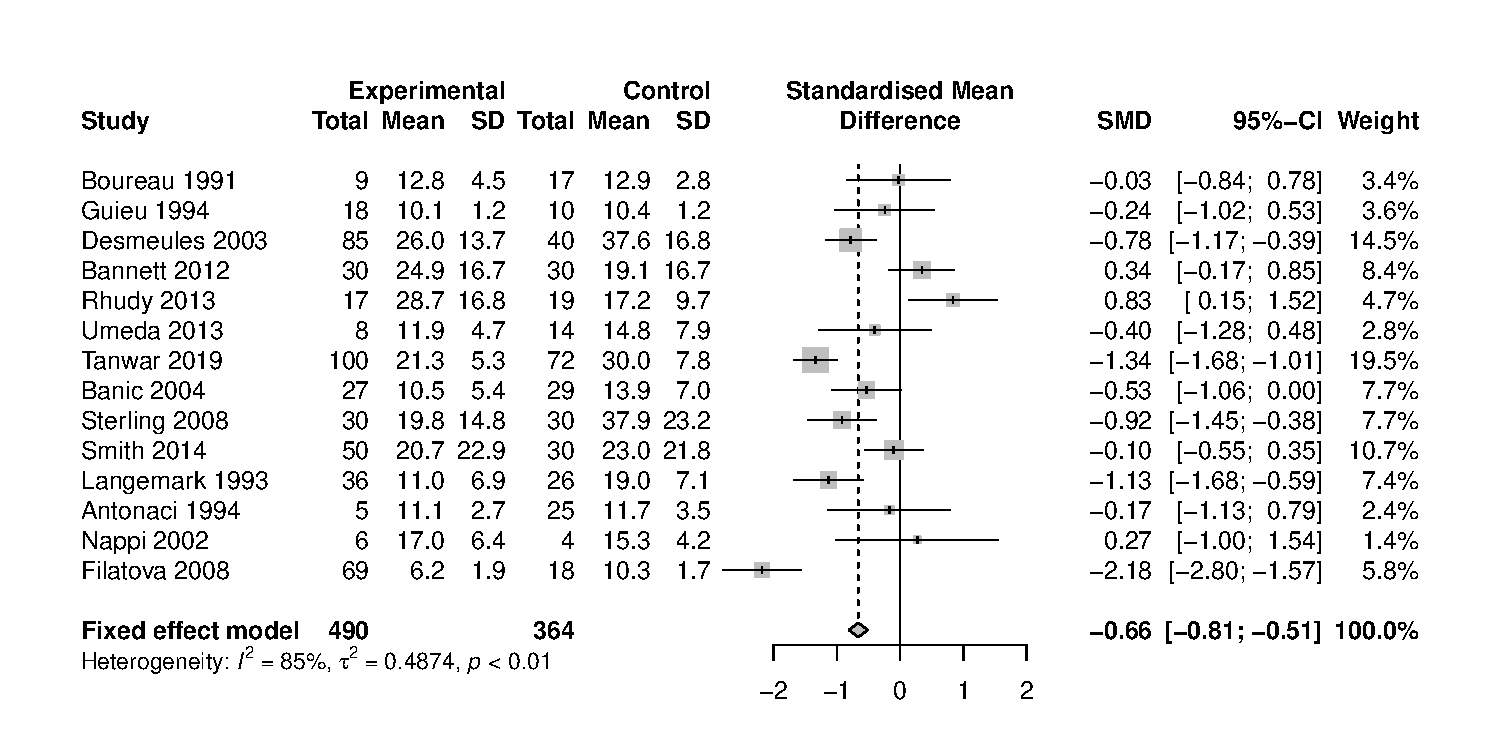
\includegraphics{IntroToMA_pdf_files/figure-latex/unnamed-chunk-1-1} 

}

\caption{Forest Plot Using meta Package}\label{fig:unnamed-chunk-1}
\end{figure}

\hypertarget{funnel-plot-using-metafor-package}{%
\subsection{Funnel Plot Using metafor Package}\label{funnel-plot-using-metafor-package}}

A \href{https://en.wikipedia.org/wiki/funnel\%20plot}{funnel plot} shows the observed effect sizes or outcomes on the x-axis against a precision measure of the observed effect sizes on the y-axis. In metafor package, the recommended choice for the y-axis is the standard error (in decreasing order) which is in line with \protect\hyperlink{ref-Sterne2001}{Sterne \& Egger} (\protect\hyperlink{ref-Sterne2001}{2001}). If there is no publication bias or heterogeneity among studies, the expectation is to see all points to fall within the pseudo-confidence shape funnel, i.e., the triangle shape funnel for the case of standard errors on the y-axis.

\begin{Shaded}
\begin{Highlighting}[]
\FunctionTok{funnel}\NormalTok{(res, }\AttributeTok{main =} \StringTok{"Standard Error"}\NormalTok{)}
\end{Highlighting}
\end{Shaded}

\begin{figure}

{\centering 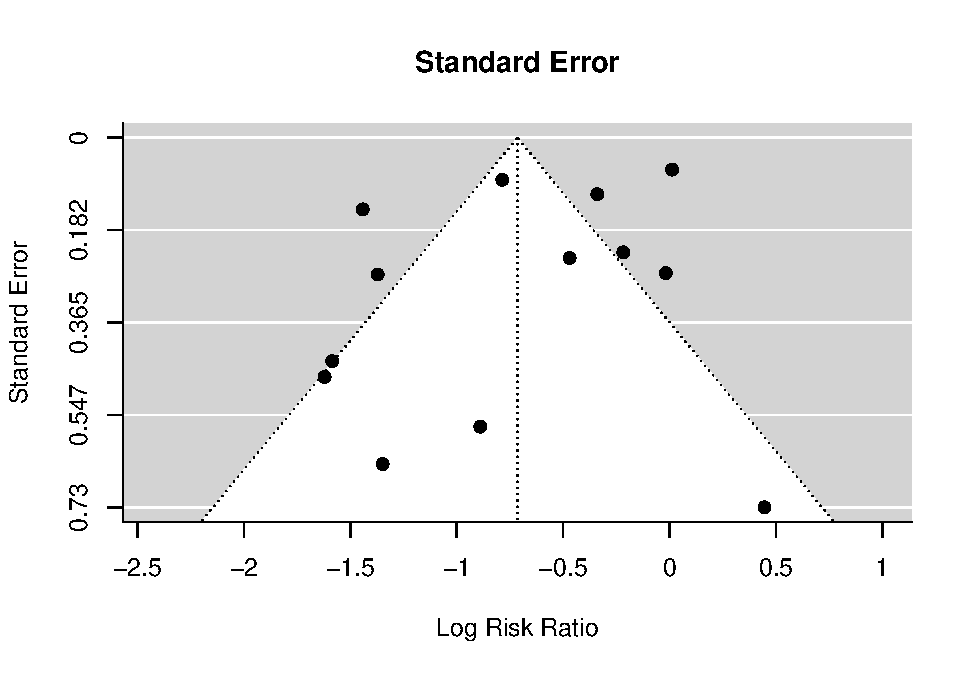
\includegraphics{IntroToMA_pdf_files/figure-latex/funnel-plot-1} 

}

\caption{Common Funnel Plots}\label{fig:funnel-plot-1}
\end{figure}

\begin{Shaded}
\begin{Highlighting}[]
\FunctionTok{funnel}\NormalTok{(res, }\AttributeTok{yaxis =} \StringTok{"seinv"}\NormalTok{, }\AttributeTok{main =} \StringTok{"Inverse Standard Error"}\NormalTok{)}
\end{Highlighting}
\end{Shaded}

\begin{figure}

{\centering 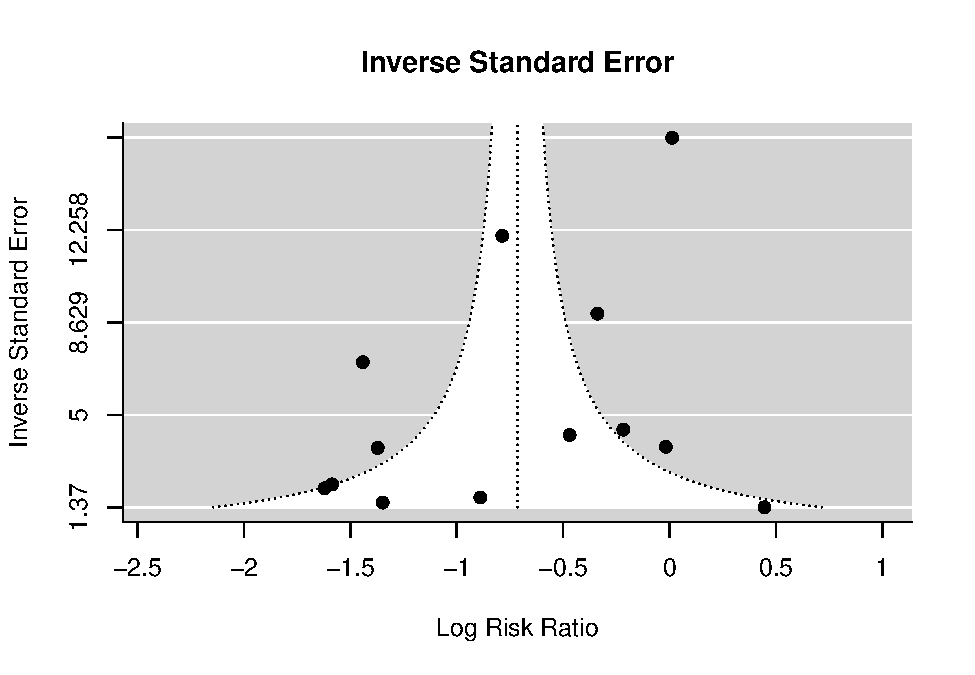
\includegraphics{IntroToMA_pdf_files/figure-latex/funnel-plot-2} 

}

\caption{Common Funnel Plots}\label{fig:funnel-plot-2}
\end{figure}

\hypertarget{funnel-plot-using-meta-package}{%
\subsection{Funnel Plot Using meta Package}\label{funnel-plot-using-meta-package}}

\begin{Shaded}
\begin{Highlighting}[]
\NormalTok{nfr }\OtherTok{\textless{}{-}} \FunctionTok{read.xlsx}\NormalTok{(}\AttributeTok{xlsxFile =} \StringTok{"NFR\_v\_Control\_final.xlsx"}\NormalTok{)}

\NormalTok{nfrModel }\OtherTok{\textless{}{-}} \FunctionTok{metacont}\NormalTok{(}\AttributeTok{data =}\NormalTok{ nfr, }\AttributeTok{n.e =}\NormalTok{ ss1, }\AttributeTok{mean.e =}\NormalTok{ m1, }\AttributeTok{sd.e =}\NormalTok{ sd1,}
    \AttributeTok{n.c =}\NormalTok{ ss2, }\AttributeTok{mean.c =}\NormalTok{ m2, }\AttributeTok{sd.c =}\NormalTok{ sd2, }\AttributeTok{studlab =}\NormalTok{ Study.Label,}
    \AttributeTok{sm =} \StringTok{"SMD"}\NormalTok{)}

\NormalTok{meta}\SpecialCharTok{::}\FunctionTok{funnel.meta}\NormalTok{(nfrModel, }\AttributeTok{contour.levels =} \FunctionTok{c}\NormalTok{(}\FloatTok{0.9}\NormalTok{, }\FloatTok{0.95}\NormalTok{, }\FloatTok{0.99}\NormalTok{),}
    \AttributeTok{yaxis =} \StringTok{"invvar"}\NormalTok{)}
\end{Highlighting}
\end{Shaded}

\begin{figure}

{\centering 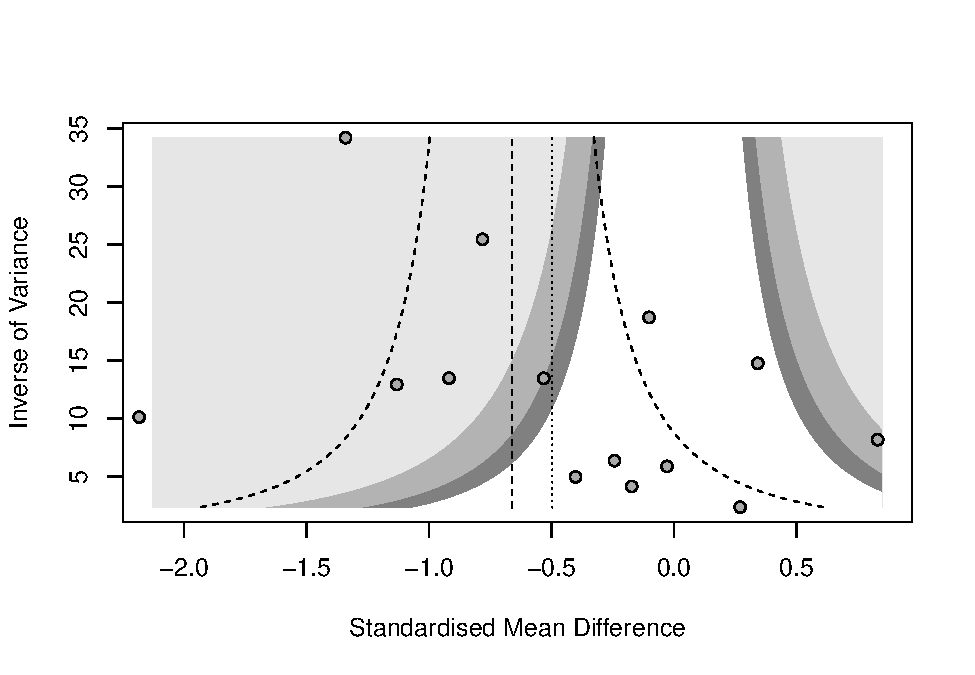
\includegraphics{IntroToMA_pdf_files/figure-latex/funnel-plot-meta-1} 

}

\caption{Common Funnel Plots Using meta Package}\label{fig:funnel-plot-meta}
\end{figure}

\hypertarget{references}{%
\section*{References}\label{references}}
\addcontentsline{toc}{section}{References}

\hypertarget{refs}{}
\begin{CSLReferences}{1}{0}
\leavevmode\vadjust pre{\hypertarget{ref-cohen1977}{}}%
Cohen, J. (1977). \emph{Statistical power analysis for the behavioral sciences}. Elsevier. \url{https://doi.org/10.1016/c2013-0-10517-x}

\leavevmode\vadjust pre{\hypertarget{ref-glass1976}{}}%
Glass, G. V. (1976). Primary, Secondary, and Meta-Analysis of Research. \emph{Educational Researcher}, \emph{5}(10), 3--8. \url{https://doi.org/10.3102/0013189x005010003}

\leavevmode\vadjust pre{\hypertarget{ref-lipsey2001}{}}%
Lipsey, M. W., \& Wilson, D. B. (2001). \emph{Practical meta-analysis.} SAGE publications, Inc.

\leavevmode\vadjust pre{\hypertarget{ref-Ruxfccker2009}{}}%
Rücker, G., Schwarzer, G., Carpenter, J., \& Olkin, I. (2009). Why add anything to nothing? The arcsine difference as a measure of treatment effect in meta-analysis with zero cells. \emph{Statistics in Medicine}, \emph{28}(5), 721--738. \url{https://doi.org/10.1002/sim.3511}

\leavevmode\vadjust pre{\hypertarget{ref-Sterne2001}{}}%
Sterne, J. A. C., \& Egger, M. (2001). Funnel plots for detecting bias in meta-analysis. \emph{Journal of Clinical Epidemiology}, \emph{54}(10), 1046--1055. \url{https://doi.org/10.1016/s0895-4356(01)00377-8}

\leavevmode\vadjust pre{\hypertarget{ref-metafor}{}}%
Viechtbauer, W. (2010). Conducting meta-analyses in r with the metafor package. \emph{Journal of Statistical Software}, \emph{36}(3), 1--48.

\leavevmode\vadjust pre{\hypertarget{ref-Yusuf1985}{}}%
Yusuf, S., Peto, R., Lewis, J., Collins, R., \& Sleight, P. (1985). Beta blockade during and after myocardial infarction: An overview of the randomized trials. \emph{Progress in Cardiovascular Diseases}, \emph{27}(5), 335--371. \url{https://doi.org/10.1016/s0033-0620(85)80003-7}

\end{CSLReferences}

\end{document}
